

\begin{table}[ht]
	\centering
	\begin{tabular}{lll}
		\toprule
		カラム名        & 単位 & データ型  \\
		\midrule
		bdaddress   & なし & str   \\
		x           & m  & float \\
		y           & m  & float \\
		floor\_name & なし & str   \\
		\bottomrule
	\end{tabular}
	\caption{BLEビーコン基地局 DF}
\end{table}


\begin{table}[ht]
	\centering
	\begin{tabular}{lll}
		\toprule
		カラム名        & 単位      & データ型  \\
		\midrule
		ts          & s (秒)   & float \\
		x           & m(メートル) & float \\
		y           & m(メートル) & float \\
		z           & m(メートル) & float \\
		bdaddress   & なし      & str   \\
		rssi        & dBm     & int   \\
		floor\_name & なし      & str   \\
		\bottomrule
	\end{tabular}
	\caption{BLEビーコンFPのDF}
\end{table}


\begin{figure}[ht]
	\centering
	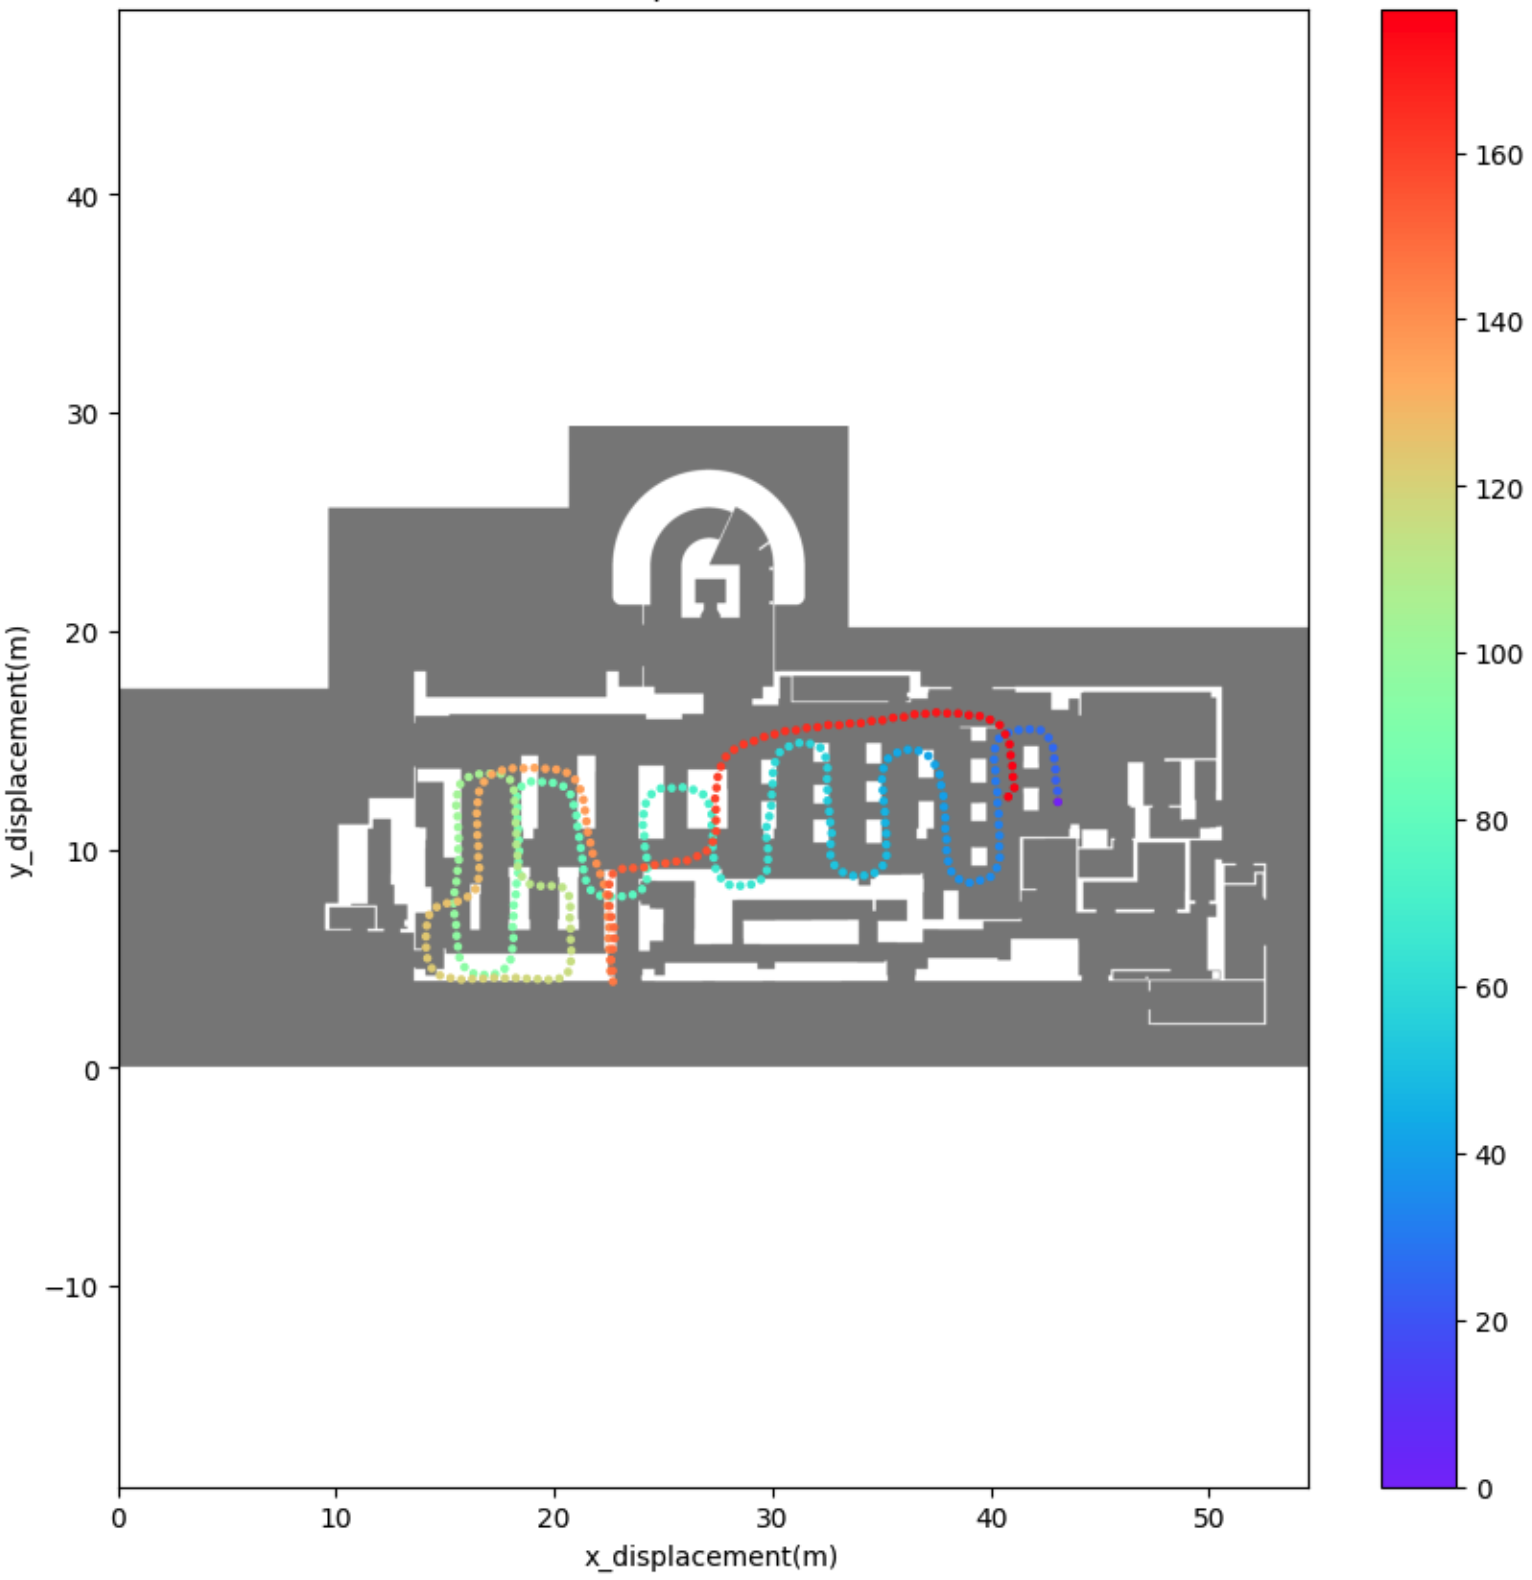
\includegraphics[width=80mm]{image/fingerprint-rotate.jpg}
	\caption{回転後の軌跡}    \label{fig:fingerprint-rotate}
\end{figure}


\begin{lstlisting}[caption={BLEビーコンのFPを使用した初期方向補正}, label=lst:rotate-trajectory-using-ble-fingerprint]
def rotate_trajectory_to_optimal
          _alignment_using_ble_fingerprint(
    acc_df: pd.DataFrame,
    angle_df: pd.DataFrame,
    ble_scans_df: pd.DataFrame,
    ble_fingerprint_df: pd.DataFrame,
    floor_name: str,
    *,
    ground_truth_first_point: dict[Axis2D, float] | None = None,
) -> tuple[pd.DataFrame, pd.DataFrame]:
\end{lstlisting}